\documentclass[a4paper,14pt]{book}
\usepackage[T1]{fontenc}
\usepackage[utf8x]{inputenc}
\usepackage[english,russian]{babel}
\usepackage{graphicx}


% \usepackage{microtype}
% \DisableLigatures{encoding=*,family=*}
% \usepackage{newunicodechar}
% \newunicodechar{ff}{ff}
% \newunicodechar{fi}{fi}
% \newunicodechar{fl}{fl}
% \newunicodechar{ffi}{ffi}
% \newunicodechar{ffl}{ffl}
\usepackage{hyperref}
\usepackage{imakeidx}



\usepackage{geometry} % Меняем поля страницы
\geometry{left=2cm}% левое поле
\geometry{right=1.5cm}% правое поле
\geometry{top=1cm}% верхнее поле
\geometry{bottom=2cm}% нижнее поле

\renewcommand{\theenumi}{\arabic{enumi}}% Меняем везде перечисления на цифра.цифра
\renewcommand{\labelenumi}{\arabic{enumi}}% Меняем везде перечисления на цифра.цифра
\renewcommand{\theenumii}{.\arabic{enumii}}% Меняем везде перечисления на цифра.цифра
\renewcommand{\labelenumii}{\arabic{enumi}.\arabic{enumii}.}% Меняем везде перечисления на цифра.цифра
\renewcommand{\theenumiii}{.\arabic{enumiii}}% Меняем везде перечисления на цифра.цифра
\renewcommand{\labelenumiii}{\arabic{enumi}.\arabic{enumii}.\arabic{enumiii}.}% Меняем везде перечисления на цифра.цифра

\usepackage{hyperref}

\begin{document}


\addcontentsline{toc}{chapter}{Права}

Copyright \textcopyright2011 Фонд OpenFOAM.

Разрешение предоставлено копировать, распространять и/или изменять этот документ согласно пунктам из GNU
 Свободной Лицензии Документации, Версия 1.2, изданная Фондом Свободного Программного обеспечения; без Неизменяемых Секций,
 никаких обложек Текстов Обратной стороны и ни одной Лицевой Обложки Текста (охраняемых этой лицензией):
“Доступно свободно на сайте ”openfoam.org”. Копия лицензии включена в секцию названную “GNU Свободная Лицензия Документации”.

Этот документ распространен в надежде, что будет полезен, но БЕЗ КАКОЙ-ЛИБО ГАРАНТИИ; без даже подразумеваемой гарантии
 ВЫСОКОГО СПРОСА или ПРИГОДНОСТИ В ПРИКЛАДНЫХ ЦЕЛЯХ.

Набран в LATEX.
\chapter{Введение}
\label{chap:1}
Это руководство сопровождает выпуск версии 2.1.0 Open Source Field Operation And Manipulation (OpenFOAM) 
(операции и манипуляции с полями с открытым исходным кодом) C++ библиотек. Оно предоставляет описание основных операций
 с OpenFOAM, сначала посредством ряда примеров руководства в \autoref{chap:2} и далее с использованием более детальных описаний 
индивидуальных компонент, которые составляют пакет OpenFOAM.
OpenFOAM это во-первых и прежде всего \textit{библиотеки на C++}, использованные сначала для создания исполняемых модулей 
(executables), называемых как \textit{приложения} (\textit{applications}). Приложения разделяются на две категории:
 решатели или \textit{солверы} (\textit{solvers}), каждый из которых создан чтобы решить частную задачу в механике сплошной
 среды; и сервисные программы или \textit{утилиты} (\textit{utilities}), которые разрабатывались для выполнения задач
 включающих обработку данных.  Дистрибутив OpenFOAM содержит многочисленные решатели и утилиты обеспечивающие
 решение широкого диапазона задач, как описано в \autoref{chap:3}.
Одна из наиболее сильных возможностей OpenFOAM заключается в том, что новые решатели и утилиты могут быть созданы его
 пользователями с некоторыми предварительными, минимально необходимыми знаниями основных использованных методов физики
 и методов программирования.
OpenFOAM поставляется с вычислительной средой включающей  пре- и постпроцессор. Интерфейс (связь с) пре- и постпроцессором
 обеспечивается утилитами OpenFOAM, таким образом гарантируя совместимость обращения с данными для всей вычислительной среды.
 Общая структура OpenFOAM показана на Рис 1.1. ( Figure 1.1.) Обработка предпроцессором и запуск кейса
OpenFOAM представлен в \autoref{chap:4}.
\begin{figure}[ht]
 \centering
 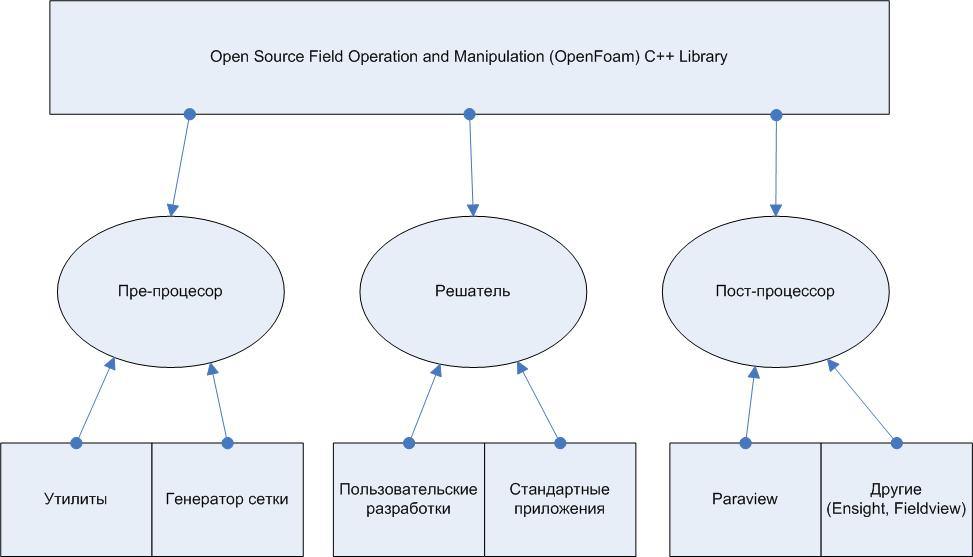
\includegraphics[width=531pt,height=273pt]{UGFigure1-1.PNG}
 UGFigure 1-1.PNG: 973x557 pixel, 96dpi, 25.74x14.74 cm, bb=0 0 730 418
 \label{fig:1.1}
 \caption{Рисунок 1.1: Условная структура пакета}
\end{figure}

 В \autoref{chap:5} мы представили как  генерацию (создание) сеток, используя  утилиты генерации сеток
 поставляемых с OpenFOAM, так и преобразование сеточных данных, созданных c использованием сторонних продуктов.
 Постпроцессорная обработка решения описана в \autoref{chap:6}.
\chapter{Учебные примеры}
В этой главе мы опишем подробно процесс установки, моделирования и пост- процесорной обработки для некоторых тестовых
 примеров OpenFOAM, с основной целью: познакомить пользователя с основными процедурами работы и управления OpenFOAM.
 \textit{\$FOAM\_TUTORIALS} директория содержит много тестовых случаев, которые демонстрируют использование всех
 решателей и многих утилит поставляемых с OpenFOAM. Прежде чем пытаться использовать обучающие программы, пользователь
 должен предварительно удостовериться  в том, что он установил OpenFOAM правильно.

Обучающие примеры описывают использование утилиты \textsl{blockMesh} - инструмента предпроцессорной обработки, установки 
примера и запуска на счет решателя OpenFOAM и постпроцессорной обработки с использованием \textsl{paraFoam}.
 Те пользователи, которые имеют доступ к постпроцессорам, разработанным другими фирмами (из инструментария посторонних
 разработчиков), также поддерживаемых в OpenFOAM, имеют выбор: либо они могут следовать за примерами обучающих программ,
 используя \textsl{paraFoam}; либо обратиться к описанию использования продукта постороннего разработчика, как описано в
главе 6, когда требуется постпроцессорная обработка.

Копии всех обучающих программ доступны в директории \textit{tutorials} из поставки OpenFOAM.
Обучающие программы организованы
 в виде ряда директорий согласно типу течения в которых расположены поддиректории согласно решателю. Например,
 все \textsl{icoFoam} примеры хранятся в пределах подкаталога \textit{incompressible/icoFoam}, где \textit{incompressible}
(несжимаемое)  указывает на тип рассматривваемого течения. Если пользователь желает запустить на расчет несколькотестовых 
примеров,  рекомендуется, чтобы пользователь сначала скопировал директорию \textit{tutorials} в свою локальноую директорию
\textit{run}. Они могут быть легко скопированы набором:

\texttt{mkdir –p \$FOAM\_RUN}

\texttt{cp –r \$FOAM\_TUTORIALS \$FOAM\_RUN}

\section{Течение в прямоугольной полости, инициированное верхней плитой}
\label{sec:2.1}
Этот раздел руководства описывает как выполнить этапы пре-процессор, расчет и постпроцессорную обработку для тестового
 примера, рассматривающего изотермическое течение несжимаемой среды в двумерной квадратной области. Геометрия течения
изображена на Рис. 2.1, в которой все границы квадрата являются стенками. Верхняя стенка перемещается в
\textit{x}-направлении со скоростью 1 м/с, в то время как другие 3 неподвижны. Первоначально принято, что будет
 рассматриваться ламинарное течение и задача будет решаться на однородной сетке, используя решатель \textsl{icoFoam}
 для ламинарного, изотермического, несжимаемого потока. В течение курса обучающей программы, будут исследованы влияние
 увеличения числа узлов сетки на решение и влияние измельчения шага сетки по направлению к стенкам.
Наконец, число Рейнольдса будет увеличено, и решатель \textsl{pisoFoam} будет использоваться для турбулентного,
 изотермического, несжимаемого течения.

\begin{figure}[h]
 \centering
 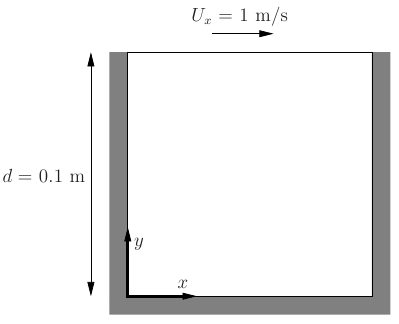
\includegraphics[width=299pt,height=243pt]{UGFigure2-1.PNG}
 % UGFigure2-1.PNG: 399x324 pixel, 96dpi, 10.56x8.57 cm, bb=0 0 299 243
 \caption{Геометрия течения в каверне, инициированного движением верхней плиты.}
 \label{fig:2.1}
\end{figure}

\section{Пре- процессорная подготовка (pre-processing)}
\label{sec:2.1.1}

В составе дистрибутива OpenFOAM поставляются примеры. Для редактирования файлов примера пользователь должен выбрать
 xeditor или другой редактор , типа \textbf{emacs}, \textbf{vi}, \textbf{gedit}, \textbf{kate}, \textbf{nedit},
 и т.п. Редактирование файлов возможно в OpenFOAM, потому что ввод / вывод использует формат словаря с ключевыми
 словами, которые представляют смысловое значение, чтобы быть понятными даже наименее опытным пользователям.

Моделируемый случай включает данные для сетки, полей, свойств, параметров контроля решения, и т.д.
 Как описано в секции 4.1, в OpenFOAM эти данные хранятся в ряде файлов в пределах директории примера,
 а не в единственном файле примера, как во многих других пакетах вычислительной гидродинамики (CFD).
 Директории примера дают соответственно описательное название, например первый случай для этого
 обучающего примера просто назван \textsl{cavity} (каверна). В подготовке редактирования файлов примера и
 запуска первого примера \textsl{cavity}, пользователь должен перейти в каталог примера

\texttt{cd \$FOAM\_RUN/tutorials/incompressible/icoFoam/cavity}

\subsection{Генерация сетки}
\label{sec:2.1.1.1}

OpenFOAM всегда работает в 3 мерной декартовой системе координат и все геометрические конфигурации производятся
 в 3 измерениях. OpenFOAM решает примеры в 3 измерениях по умолчанию, но может быть проинструктирован решать
 в 2 измерениях, определяя специальное \textsl{empty} (пустое) граничное условие на границах, нормальных к (3-ему)
 z измерению (для данного примера), для которого никакое решение проводить не требуется.
Область примера \textsl{cavity} состоит из квадрата c длинами сторон \textit{d} = 0.1 м. в \textit{x-y} плоскости.
Первоначально будет использоваться равномерная сетка 20 на 20 ячеек. В блочной конструкции показанной на Рис. 2.2. генератор сеток,
 поставляемый с OpenFOAM, \textit{blockMesh}, создает сетки, используя команды из описания определенного в словаре ввода,
 \textit{blockMeshDict} расположенного в каталоге \textit{constant/polyMesh} данного примера. Чтобы перейти к
 \textit{blockMeshDict}  для этого примера  возьмем следующий файл:
\begin{verbatim}
/*--------------------------------*- C++ -*----------------------------------*\
| =========                 |                                                 |
| \\      /  F ield         | OpenFOAM: The Open Source CFD Toolbox           |
|  \\    /   O peration     | Version:  2.1.0                                 |
|   \\  /    A nd           | Web:      www.OpenFOAM.com                      |
|    \\/     M anipulation  |                                                 |
\*---------------------------------------------------------------------------*/
FoamFile
{
    version     2.0;
\end{verbatim} 

\begin{figure}[h]
 \centering
 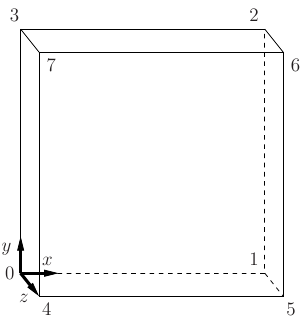
\includegraphics[width=229pt,height=241pt]{UGFigure2-2.PNG}
 % UGFigure2-2.PNG: 306x321 pixel, 96dpi, 8.10x8.49 cm, bb=0 0 229 241
 \caption{Блочная конструкция сетки для каверны.}
 \label{fig:2.2}
\end{figure}

\begin{verbatim}
    format      ascii;
    class       dictionary;
    object      blockMeshDict;
}
// * * * * * * * * * * * * * * * * * * * * * * * * * * * * * * * * * * * * * //

convertToMeters 0.1;

vertices        
(
    (0 0 0)
    (1 0 0)
    (1 1 0)
    (0 1 0)
    (0 0 0.1)
    (1 0 0.1)
    (1 1 0.1)
    (0 1 0.1)
);

blocks          
(
    hex (0 1 2 3 4 5 6 7) (20 20 1) simpleGrading (1 1 1)
);

edges           
(
);

boundary
(
    movingWall 
    {
        type wall;
        faces
        (
            (3 7 6 2)
        );
    }
    fixedWalls 
    {
        type wall;
        faces
        (
            (0 4 7 3)
            (2 6 5 1)
            (1 5 4 0)
        );
    }
    frontAndBack 
    {
        type empty;
        faces
        (
            (0 3 2 1)
            (4 5 6 7)
        );
    }
);

mergePatchPairs 
(
);

// ************************************************************************* //

\end{verbatim}

В начале файла содержится заголовок в форме баннера (строки 1-7), далее информация файла
 содержится в подсловаре \textsl{FoamFile}, заключенная в фигурных скобках ({...}).

\textit{В остальной части руководства:}
Ради сохранения места и для ясности, шапка или заголовок файла, включая баннер и \textsl{FoamFile} подсловарь,
 и обрамление в скобках не будут включаться в файлы примеров.

Файл в начале содержит блок вершин \texttt{vertices} (x,y,z координаты точек); затем в нем определяются сами блоки
 (\texttt{blocks})  (в данном примере имеется только 1) с помощью описанных выше меток вершин и номеров
 ячеек внутри них; и наконец, в файле определяются поверхности для задания граничных патчей.
 Пользователю предлагается обратиться к секции 5.3 чтобы понять значение вводимых  величин в \textsl{blockMeshDict} файле.

Сетка генерируется при запуске утилиты \textsl{blockMesh}, использующей файл \textsl{blockMeshDict}.
Запуск производится из директории задачи, просто набором команды в терминале:

\texttt{blockMesh}

Состояние выполнения \textsl{blockMesh} выводится в окне терминала. Любые ошибки в исходном 
файле сетки \textsl{blockMeshDict} обрабатываются textsl{blockMesh} и итоговые сообщения об ошибках показывают 
пользователю номер строки в которой возникла проблема. На этой стадии не должно быть никаких сообщений об ошибках.

\subsection{Граничные и начальные условия}
\label{sec:2.1.1.2}

\chapter{N}
\chapter{N}
\chapter{Создание и конвертация сеток}

Эта глава описывает все вопросы, связанные с созданием сеток в пакете OpenFOAM:
Раздел 5.1 даёт обзор путей, которыми может быть описана сетка в OpenFOAM;
 Раздел 5.3 охватывает подпрограмму blockMesh для генерации простых сеток из
блоков
гексаэдрических элементов; Раздел 5.4 охватывает подпрограмму snappyHexMesh для
автоматического создания сложных сеток из гексаэдрических и расщеплённых
гексаэдрических элементов из
 триангулированных геометрических поверхностей; раздел
5.5 описывает имеющиеся опции для конвертации сетки, созданной в других пакетах,
в формат, доступный для чтения OpenFOAM.

\section{Описание сетки}
\label{sec:5.1}

Этот раздел раскрывает описание классов OpenFOAM С++, работающих с сеткой.
Сетка является составной частью численного расчёта и должна удовлетворять
определённому
 критерию для получения качественного и точного результата. В процессе
запуска, OpenFOAM проверяет соответствие сетки набору строгих ограничений и
завершит
 работу, если ограничения не будут соблюдены. Это важно, потому что пользователь
 перед запуском OpenFOAM может некорректно исправить большую сетку
в программах сторонних разработчиков. Это является некоторым недостатком, но
мы (разработчики) не оправдываем OpenFOAM просто усваивая хорошие примеры
из практики. Убедитесть в том, что сетка соответствует требованиям расчёта; в
ином
случае решение будет некорректным уже перед запуском программы.
По умолчанию OpenFOAM определяет 3D сетку из случайных многогранников,
ограниченных случайными полигональными гранями, т.е. элементы могут иметь
бесконечное количество поверхностей, в которых, для каждой поверхности, имеется
 неограниченное количество рёбер и нет ограничений на их положение. Сетка с
такой
 общей структурой известна в OpenFOAM как polyMesh. Детально она
описывается в разделе 2.1 Руководства программиста, но важно запомнить, что
этот тип сетки позволяет получить большую свободу при создании и манипуляции
с сетками, в частности когда геометрия домена сложна, либо изменяется во времени.
 Ценой такой универсальности сетки является сложность её генерации с помощью
 программ-преобразователей. Поэтому в OpenFOAM предусмотрена утилита
cellShape для управления общепризнанными форматами сеток, основанных на множестве
 предопределённых форм элементов.

\subsection{Описание сетки и её применимость}

Перед описанием OpenFOAM-формата сетки, polyMesh, и утилит cellShape, мы, в
первую очередь, установим критерии применимости, используемые в OpenFOAM.
Условия, которым должна удовлетворять сетка даны ниже:

\subsubsection{Точки}

Точка является областью 3D пространства, определяемой вектором в метрах. Точки
компилируются в список и каждая точка связывается с указателем, который обозначает её
 позицию в списке, начинающемся с нуля. Список точек не может содержать
две точки, обладающие совершенно идентичным расположением, так же как точку,
не принадлежащую по крайней мере одной грани.

\subsubsection{Грани}

Грань - это упорядоченный список точек, в котором каждая точка имеет свою метку.
Упорядочивание меток точек происходит из условия того, чтобы две соседние точки
 были соединены ребром, т.е. следуя нумерации вы перебираете точки, обходя по
кругу грани. Грани компилируются в список и каждая грань имеет свою метку, отображающую
 её положение в списке. Направление вектора нормали грани выбирается
по правилу правой руки, т.е. при взгляде по направлению к грани, если нумерация
точек идёт против часовой стрелки, нормаль направлена к Вам, как показано на
рисунке 5.1.





\end{document}
